\chapter{Attacks}
\label{chapter:attacks}
Various attacks has been performed against Bitcoin in the past.
Attacks can be performed at different levels with very different approaches and can have a wide range of effects on Bitcoin users.
This chapter starts from an overview of the most relevant ones.
At the end, it describes in details the Balance attack, whose analysis is the main object of the simulations.

\section{Double Spending}
Double-spending is the result of successfully spending some money more than once.
The attack is the oldest known one against Bitcoin (it is even partially discussed in the original Bitcoin paper \cite{bitcoin_2009}).
The attack has been analyzed many times in the literature \cite{double_spending_fast_payments, double_spending_two_for_one, double_spending_bitcoin_economics, double_spending_fast_analysis_2014} and has been reported to be quite easy to mount for fast payments \cite{double_spending_fast_payments}.
Real episodes of the attack has been reported multiple times in the past \cite{double_spending_ghash, double_spending_stackexchange}.
Double-spending breaks the most important guarantee that Bitcoin tries to give:
transactions are irreversible and bitcoins can be spent only once.

The attack works by creating \num{2} conflicting transactions (that spend all the bitcoins in the same address) and submitting them to different parties, for example \texttt{tx-1} to a merchant and \texttt{tx-2} to the Bitcoin network:
if the merchant accepts \texttt{tx-1} but the Bitcoin network receives \texttt{tx-2} before \texttt{tx-1}, it is likely that \texttt{tx-2} will be stored in the blockchain, while \texttt{tx-1} will be discarded, since not compatible with \texttt{tx-2}.
The attacker only pretends to spend some bitcoins to pay the merchant, but it actually does not spend anything:
it gets the purchase for free, while the merchant never receives the due bitcoins.
The double-spending attack can be performed directly in some cases, or it can be the result of more complex attacks.
There are many variants of double-spending, we analyze the most common ones here.

\subsection{Race Attack}
\label{sub:race-attack}
The race attack involves merchants that immediately accepts payments, without waiting for the unconfirmed transaction to be securely store in some block in the blockchain \cite{bitcoin_wiki_irreversible_transactions}.
The race attack has a high degree of success for an attacker \cite{double_spending_two_for_one}.
The attack is illustrated in \cref{fig:race-attack} and works as follows:
\begin{itemize}
	\item the attacker sends a transaction \texttt{tx-1} to the merchants;
	\item at the same time, the attacker sends a conflicting transaction \texttt{tx-2} to some miner; the conflicting transaction spend the bitcoins stored in the same address used in \texttt{tx-1} and sends them to new address in control of the attacker;
	\item the merchants sees the unconfirmed transaction and accepts the payment; this scenario is more likely for in-shop purchases, where, in many cases, the merchant can not wait for the transaction to be stored in the blockchain;
	\item \texttt{tx-2} is received before \texttt{tx-1} from the miners, so it is more likely to be stored in some block before \texttt{tx-1};
	\item \texttt{tx-2} is stored in a block, while \texttt{tx-1} is rejected since in conflict with \texttt{tx-1}.
	      % \item the attacker receives its bitcoins back, while the merchant does not get anything.
\end{itemize}

\begin{figure}[t]
	\centering
	\vspace*{0.25cm}
	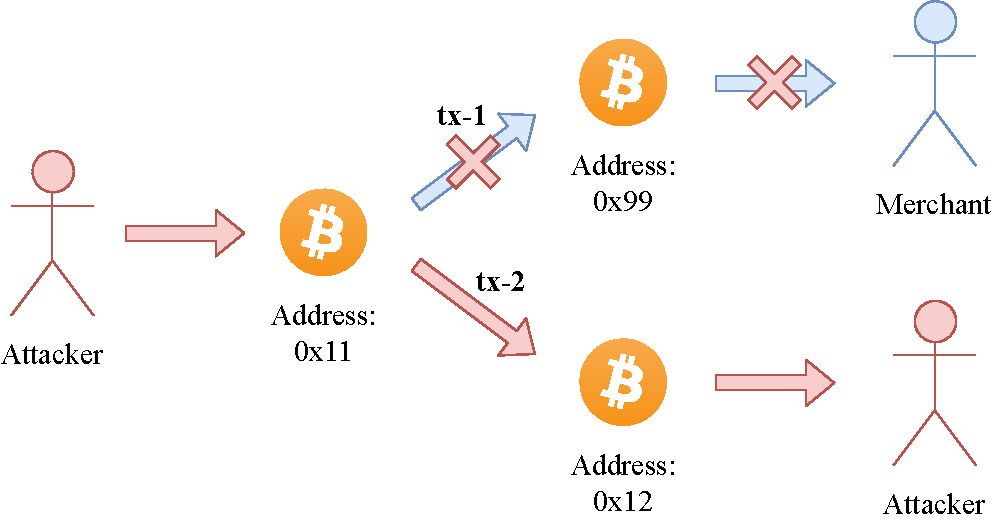
\includegraphics[scale=0.75]{figures/race_attack}
	\vspace*{0.25cm}
	\caption{
		Illustration of the race attack, a variant of double-spending.
		The attacker (in red) owns some bitcoins in the address \texttt{0x11}.
		It submits a transaction \texttt{tx-1} to move the money from its address \texttt{0x11} to the merchant's one \texttt{0x99} (in blue).
		At the same time, it submit to the Bitcoin network a conflicting transaction \texttt{tx-2} to move the the money from \texttt{0x11} to a new address \texttt{0x12} in its control.
		If the network includes \texttt{tx-2} in some block before \texttt{tx-1}, \texttt{tx-1} is rejected, and the money stay control of the attacker.
		The color of the arrows indicates the real flow of bitcoins, after that \texttt{tx-2} is stored in the blockchain and \texttt{tx-1} is rejected.
	}
	\label{fig:race-attack}
\end{figure}

A trivial defense for the merchant is to wait for the transaction \texttt{tx-1} to be stored in the blockchain:
if it is rejected because of any conflicts, the merchant can simply refuse the payment and do not sell the good.
Unfortunately, Bitcoin requires on average \SI{10}{minutes} to confirm a transaction, so this technique can not be always applied.
Bitcoin's developers recommendation is to wait for \num{6} confirmations, i.e. to wait for the block that stored the transaction to be in the longest chain and to have \num{6} following blocks \cite{confirmation}.
Some blocks can be conflicting with each other (if they have the same parent):
only one of them can belong to the longest chain, while the others are said to be ``orphaned'' \cite{orphaned_block} and simply ignored, as illustrated in \cref{fig:orphaned-block}.
Thus, a transaction can be rejected even if it manages to get part of a block, if that block is orphaned.
Waiting for \num{6} confirmations gives a good tradeoff between the time to wait (on average \SI{1}{hour}) and statistical guarantee that the transaction is unlikely to be rejected later \cite{bitcoin_2009}.

\begin{figure}[ht]
	\centering
	\vspace*{0.25cm}
	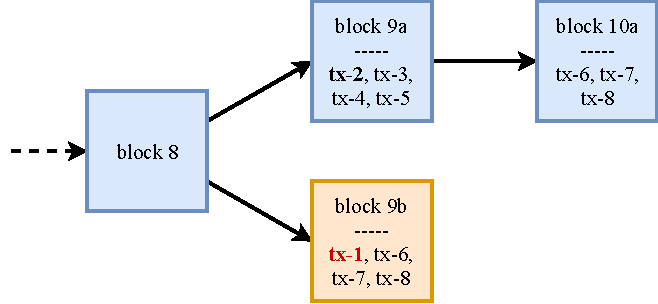
\includegraphics[scale=1.1]{figures/orphaned_block}
	\vspace*{0.25cm}
	\caption{
		Illustration of an orphaned block.
		Blocks \texttt{9a} and \texttt{9b} have the same parent.
		Since \texttt{9a} has a child \texttt{10a}, it is on the longest chain.
		Transactions \texttt{tx-6}, \texttt{tx-7} and \texttt{tx-8} from the orphaned block \texttt{9b} are stored in \texttt{10a};
		\texttt{tx-1} (in red) is in conflict with \texttt{tx-2} and is thus rejected.
	}
	\label{fig:orphaned-block}
\end{figure}

\subsection{Finney Attack}
The Finney attack is another variant of double-spending targeting merchants that accepts unconfirmed payments.
It can be performed by an attacker that is able to mine some blocks.
The attack works as follows:
\begin{itemize}
	\item the attacker controls addresses \texttt{addr-a} and \texttt{addr-b};
	\item the attacker mines a new block on the longest chain; the block includes a transactions \texttt{tx-2} that moves all bitcoins from address \texttt{addr-a} to \texttt{addr-b};
	\item before broadcasting the block to the Bitcoin network, the attacker sends a transaction \texttt{tx-1} to a merchant, spending again the bitcoins in \texttt{addr-a};
	\item as soon as the merchants accepts the payment, the attacker broadcasts its block to the network;
	\item \texttt{tx-2} is stored in the blockchain before \texttt{tx-1}, so \texttt{tx-1} is rejected because in conflict with \texttt{tx-2};
	\item the attacker receives its bitcoins back, while the merchant does not get anything.
\end{itemize}
Similarly to the Race attack, the Finney attack relies on conflicting transactions and the significant time required to confirm a transaction with a high confidence in Bitcoin.
The defense for the merchant is the same discussed in \cref{sub:race-attack}.

\section{Majority Attack}
\label{sec:majority-attack}
The majority attack, also known as \num{51}\% attack, refers to a situation in which one miner (or one group of miners) control more that \num{50}\% of the entire network's mining hash rate \cite{majority_investopedia, majority_bitcoin_wiki}.
An attacker with such a computational power can generate blocks faster than the rest of the network, so it can take control of the entire blockchain and each block in the longest chain.
The attacker strategy is to mine its private chain, ignoring the current longest chain and each block honest miner published.
This strategy gives statically guarantees to eventually generate the longest chain, no matter the advantage of honest miners (in terms of the difference in the number of blocks on the current longest chain and the number of blocks in the attacker's chain).
Such an attacker could, potentially, start its own chain from the genesis block and revert the entire history of Bitcoin, as illustrated in \cref{fig:majority-attack}.

There is no defense against this attack:
Bitcoin's security relies on an honest majority of nodes that collectively control more computational power than any attacker (or group of attackers) \cite{bitcoin_2009}.
To be more precise, the system is not vulnerable to the majority attack as long as no single coalition of miners controlling more than \num{50}\% of the total hash rate \cite{bitcoin_wiki_irreversible_transactions}.

\begin{figure}[t!]
	\begin{subfigure}{\textwidth}
		\centering
		\vspace*{0.25cm}
		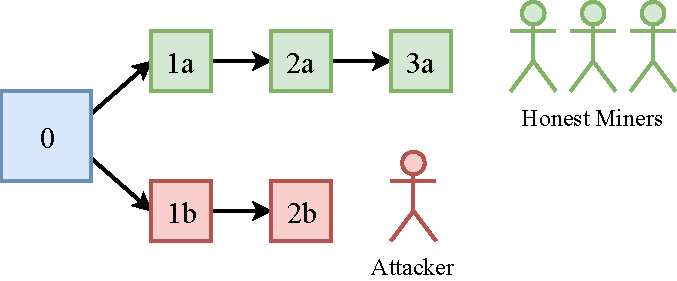
\includegraphics[scale=0.9]{figures/majority_attack_1}
		\vspace*{0.25cm}
		\caption{
			The attacker starts to mine block (in red) from the genesis (number \texttt{0}, in blue) instead of following the longest chain (in green).
			Honest miners keep following the green chain that finishes with block \texttt{3a}.
		}
		\vspace*{0.75cm}
	\end{subfigure}
	\begin{subfigure}{\textwidth}
		\centering
		\vspace*{0.25cm}
		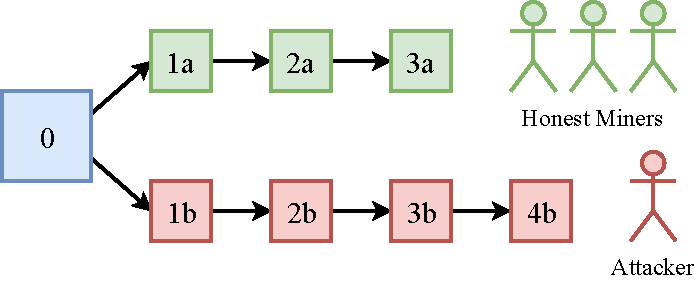
\includegraphics[scale=0.9]{figures/majority_attack_2}
		\vspace*{0.25cm}
		\caption{
			Eventually, the attacker's chain gets longer than the previous longest chain.
			The attacker broadcasts all blocks in his chain to the Bitcoin network.
		}
		\vspace*{0.75cm}
	\end{subfigure}
	\begin{subfigure}{\textwidth}
		\centering
		\vspace*{0.25cm}
		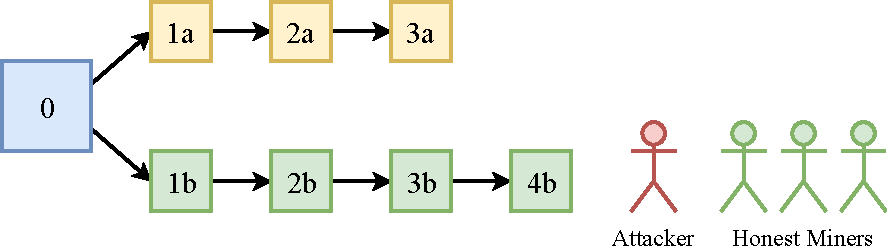
\includegraphics[scale=0.9]{figures/majority_attack_3}
		\vspace*{0.25cm}
		\caption{
			Honest miners start following the attacker's chain (now in green), since it is not longer than the chain terminating with block \texttt{3a}.
			The oldest chain (now in yellow) is orphaned: all transactions stored in blocks \texttt{1a}, \texttt{2a} and \texttt{3a} are not valid anymore.
			Potentially, the attacker may include transactions conflict with the canceled once in any of the new blocks \texttt{1b}, \texttt{2b}, \texttt{3b} and \texttt{4b}, effectively double-spending some or all of its bitcoins.
		}
		\vspace*{0.25cm}
	\end{subfigure}
	\caption{
		Illustration of the different phases of a majority attack, where an attacker takes control of the entire blockchain, starting from the genesis block.
		The attacker is able to revert the history of all transactions stored in the blockchain.
	}
	\label{fig:majority-attack}
\end{figure}

The majority attack allows an attacker to perform the following actions \cite{weaknesses_bitcoin_wiki}:
\begin{itemize}
	\item rewrite the history of the blockchain;
	\item prevent some or all transactions from becoming part of the longest chain;
	\item prevent some or all other miners from attaching new blocks to the longest chain (and thus getting any reward);
	\item reverse transactions it has made in the past, effectively double-spending its bitcoins;
	\item gain the revenue of all new blocks.
\end{itemize}

A majority attack can completely destroy the working of Bitcoin and violate some of its main guarantees (e.g. spending the same bitcoins only once).
Such an attack is thought to be very unlikely \cite{ghash_never_51_attack_cex, ghash_never_51_attack_coindesk}, because of its huge cost in terms of computing power and the risk for an attacker not to gain anything from it:
even if it is theoretically possible to revert all blocks following the genesis, it is incredible expensive.
The attack would immediately destroy the credibility of Bitcoin and has \num{2} possible effects:
\begin{enumerate}
	\item bitcoins value drops completely, and the attacker had no real reward;
	\item the rules of the software are changed by the community to revert the attack \cite{weaknesses_bitcoin_wiki}.
\end{enumerate}

% TODO: this makes formatting better...
\pagebreak

In January 2014, the mining pool \texttt{GHash.IO} reached \num{42}\% of the total Bitcoin hash rate \cite{ghash_fears_51_attack, security_survey_2017}, and later in July 2014 it exceeded the threshold of \num{51}\% \cite{wikipedia_ghash, majority_investopedia, bitcoin_wiki_irreversible_transactions}.
Even though there is no evidence of a majority attack to ever been mounted against Bitcoin, the episode was quite controversial in 2014:
a number of miners voluntarily dropped out of the pool and \texttt{GHash.IO} implemented a mechanism to prevent the situation to ever happen again in the future \cite{ghash_51_percent_extremetech, ghash_commits_to_40_percent_coindesk, ghash_commits_to_40_percent_arstechnica}.


\section{Selfish Mining}
Selfish Mining \cite{selfish_mining_acm} is a strategy where a group of miners strategically chooses when to submit the new blocks to the public chain, rather than submitting them immediately upon discovery.
The selfish miners keep the discovered blocks private, intentionally forking the blockchain and mining on their own private branch.
The honest nodes do not know about the blocks discovered by the selfish miners, so they continue to mine on the public chain.
If the public longest chain approaches the selfish miners' private branch length, they reveal some blocks to surpass the public chain again.
The selfish miners causes the honest miners to waste a lot of computational power on obsolete chains, since the longest one is not yet public.
The idea is illustrated in \cref{fig:selfish-mining}.

Selfish Mining has been proposed in 2013 by Ittay Eyal and Emin G\"un Sirer \cite{selfish_mining}.
In their paper, they show that both the selfish and the honest miners waste some resources, but the honest miners waste proportionally more:
overall, the rewards share for the selfish miners is higher than the proportion of computational power they own.
In practice, this gives the selfish miners an advantage over the others and encourages rational miners to join the group of selfish miners.
According to the paper, relatively small group of miners can adopt the selfish strategy and attract many other miners, with the risk of gaining the majority of the mining power (see \cref{sec:majority-attack}).

\begin{figure}[h]
	\begin{subfigure}{\textwidth}
		\centering
		\vspace*{0.25cm}
		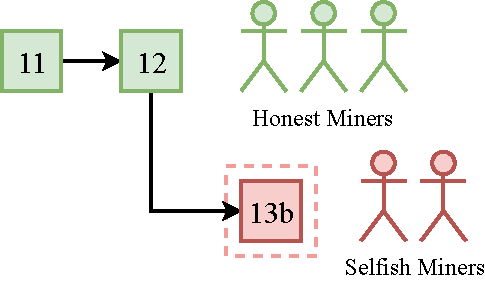
\includegraphics[scale=0.9]{figures/selfish_1}
		\vspace*{0.25cm}
		\caption{
			The selfish miners secretly mine block \texttt{13b} from the current public longest chain (in green).
			The honest miners do not know about block \texttt{13b}, so they keep working from block \texttt{12}.
		}
		\vspace*{0.75cm}
	\end{subfigure}
	\begin{subfigure}{\textwidth}
		\centering
		\vspace*{0.25cm}
		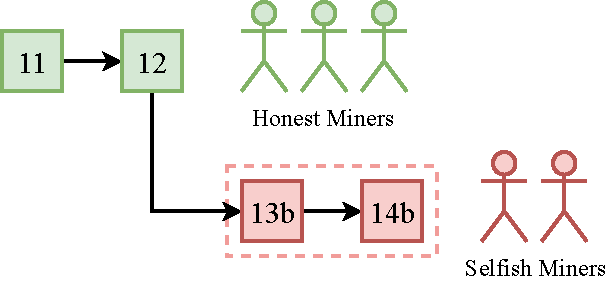
\includegraphics[scale=0.9]{figures/selfish_2}
		\vspace*{0.25cm}
		\caption{The selfish miners manage to secretly mine another block \texttt{14b} and keep it secret (secret blocks are indicated by the red dashed box).}
		\vspace*{0.75cm}
	\end{subfigure}
	\begin{subfigure}{\textwidth}
		\centering
		\vspace*{0.25cm}
		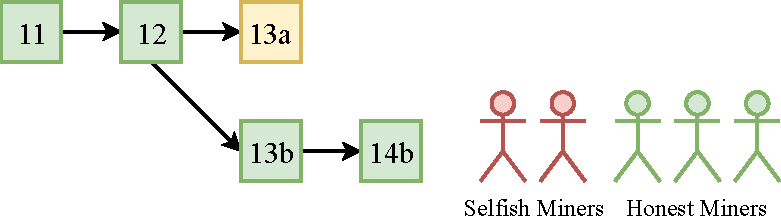
\includegraphics[scale=0.9]{figures/selfish_3}
		\vspace*{0.25cm}
		\caption{
			Honest miners manage to mine block \texttt{13a} and publish it.
			Selfish miners reveal the secret chain, which is longer than the public longest chain.
			Honest miners discard block \texttt{13a} (in yellow) and start to follow the new longest chain (block \texttt{14b}).
			The computational power used to mine block \texttt{13a} gets wasted and the honest miners do not get any revenue.
		}
		\vspace*{0.25cm}
	\end{subfigure}
	\caption{Illustration of the Selfish Mining strategy.}
	\label{fig:selfish-mining}
\end{figure}

\bigskip
Some work has been done in academics to investigate alternative mining strategy.
Nayak Kartik et at. have proposed Stubborn Mining \cite{stubborn_mining_2016}, a strategy heavily inspired by Selfish Mining, but that accepts some more risk (e.g. keep mining on chains shorter than the longest one) in return to a higher expected revenue.
They claim that stubborn mining strategies can beat Selfish Mining by up to \num{25}\%.

Ayelet Sapirshtein, Yonatan Sompolinsky and Aviv Zohar have investigated the space of possible selfish mining strategies, looking for the optimal strategy for selfish miners \cite{optimal_selfish_mining_2016}.
They also show that selfish mining strategies can be combined with double-spending attempts to make them even more profitable for selfish miners.
